\section{Proof}
Let $U $ be the Unit Disk Graph of the Euclidean Graph of a Node Set $S $.
The authors of \cite{kanj} use $LDel^{(2)}(U) $ as the underlying subgraph of the Modified Yao Step.
$LDel^{(2)}(U) $ is defined as the union of the Gabriel-graph and the subgraph of U in which the circumcircle of every triangle does not contain a 2-hop-neighbor of the nodes which create the triangle.
However, it is not known whether $LDel^{(2)}(U) $ can be constructed reactively.
At this point I want to introduce the \emph{Partial Delaunay Triangulation (PDT)} \cite{pdt} which might be a valid replacement.
The following part of this work will examine the possibility of this replacement and, thus, proving the correctness of the following proposition:

\begin{prop}
\label{mastertheorem}
Let $G $ be the PDT-subgraph of $U $.
For every integer $k \geq 14 $, there exists a subgraph $G' $ of $G $ such that $G' $ has maximum degree k and stretch factor $1+2\pi (k*\cos{\frac{\pi}{k}})^{-1} $.
\end{prop} 



With $GG $ being the Gabriel Graph, we define the Partial Delaunay Triangulation as follows:
\begin{definition}
\label{emptycircle}
An edge $UV $ is in $G $ if either 
\begin{enumerate}
\renewcommand{\labelenumi}{(\roman{enumi})}
 \item $UV \in U$ and $UV \in GG $
 \item or $\exists{W} \in U : $ maximizes $\angle{UWV} $, $\bigcirc{UVW}  \backslash \{U, V, W\} = \emptyset $ and $\sin{\angle{UWV}} \geq \frac{|CA|}{R} $, with $R>0 $ being the unit disk radius.
\end{enumerate} 
\end{definition}


Additionally, the following Delaunay Graph property is being used:
\begin{lemma}
\label{emptyregion}
If CA and CB are edges of the PDT graph then the region $R_1 $ of $(O)=\bigcirc{ABC} $ subtended by chord CA and away from B and the region $R_2 $ of $(O) $ subtended by chord CB and away from A contain no points that are two hop neighbours of A, B and C.
\end{lemma}


See Figure \ref{fig:empty_region} for a graphical illustration of the above lemma.
Let $disk(A, C) $ be the circle with $C $ and $A $ on it`s border and the middlepoint on Line $CA $.
This property also holds true for PDT.

\begin{proof}
Since $CA \in G $ either: 
\begin{enumerate}
\renewcommand{\labelenumi}{(\roman{enumi})}
\item $CA \in GG $:

$B $ cannot lie inside $disk(A, C) $. 
Therofore, $R_1 $ must be completely inside $disk(A, C) $.
\item or $CA \in G\backslash GG $ is satisfied. 

Since $CA \in G $ and $CA \notin GG $, $\exists W\in U : W$ maximizes the interior angle $\angle{CWA}  $, more specifically, $W $ is the closest node to $CA $.
There are two cases, where $W $ can be located:
\begin{enumerate}
\renewcommand{\labelenumi}{(\alph{enumi})}
\item $W $ lies in the halfplane subtended by line $CA $ away from $B $.

$W $ cannot reside in $R_1 $, since the circumcircle $\bigcirc{ACW} $ would contain $B $, which is not allowed by precondition.
Thus, $W \notin R_1 $ is true.
Therefore, $\bigcirc{ACW} $ does certainly contain $R_1 $.

\item $W $ lies in the halfplane subtended by line $CA $ towards $B $.

Since $W $ is the angle maximizing node with respect to $CA $, the following is true: $\angle{CWA} > \angle{BCA} $.
Therefore, $W \in \bigcirc{ABC} $ and since $\bigcirc{ACW} $ does not overlap $\bigcirc{ABC} $ on the side subtended by line $CA $ where $W $ is, it must overlap $\bigcirc{ABC} $ on the other side.
Thus, it must contain $R_1 $ completely.



\end{enumerate} 


\end{enumerate}


\end{proof} 



We need to show that there is a path from $A $ to $B $.
First, we divide the proof into two cases: when $\triangle{ABC} $ contains nodes of G and when this triangle is devoid of any nodes of G.

\begin{figure}[h!]
\centering
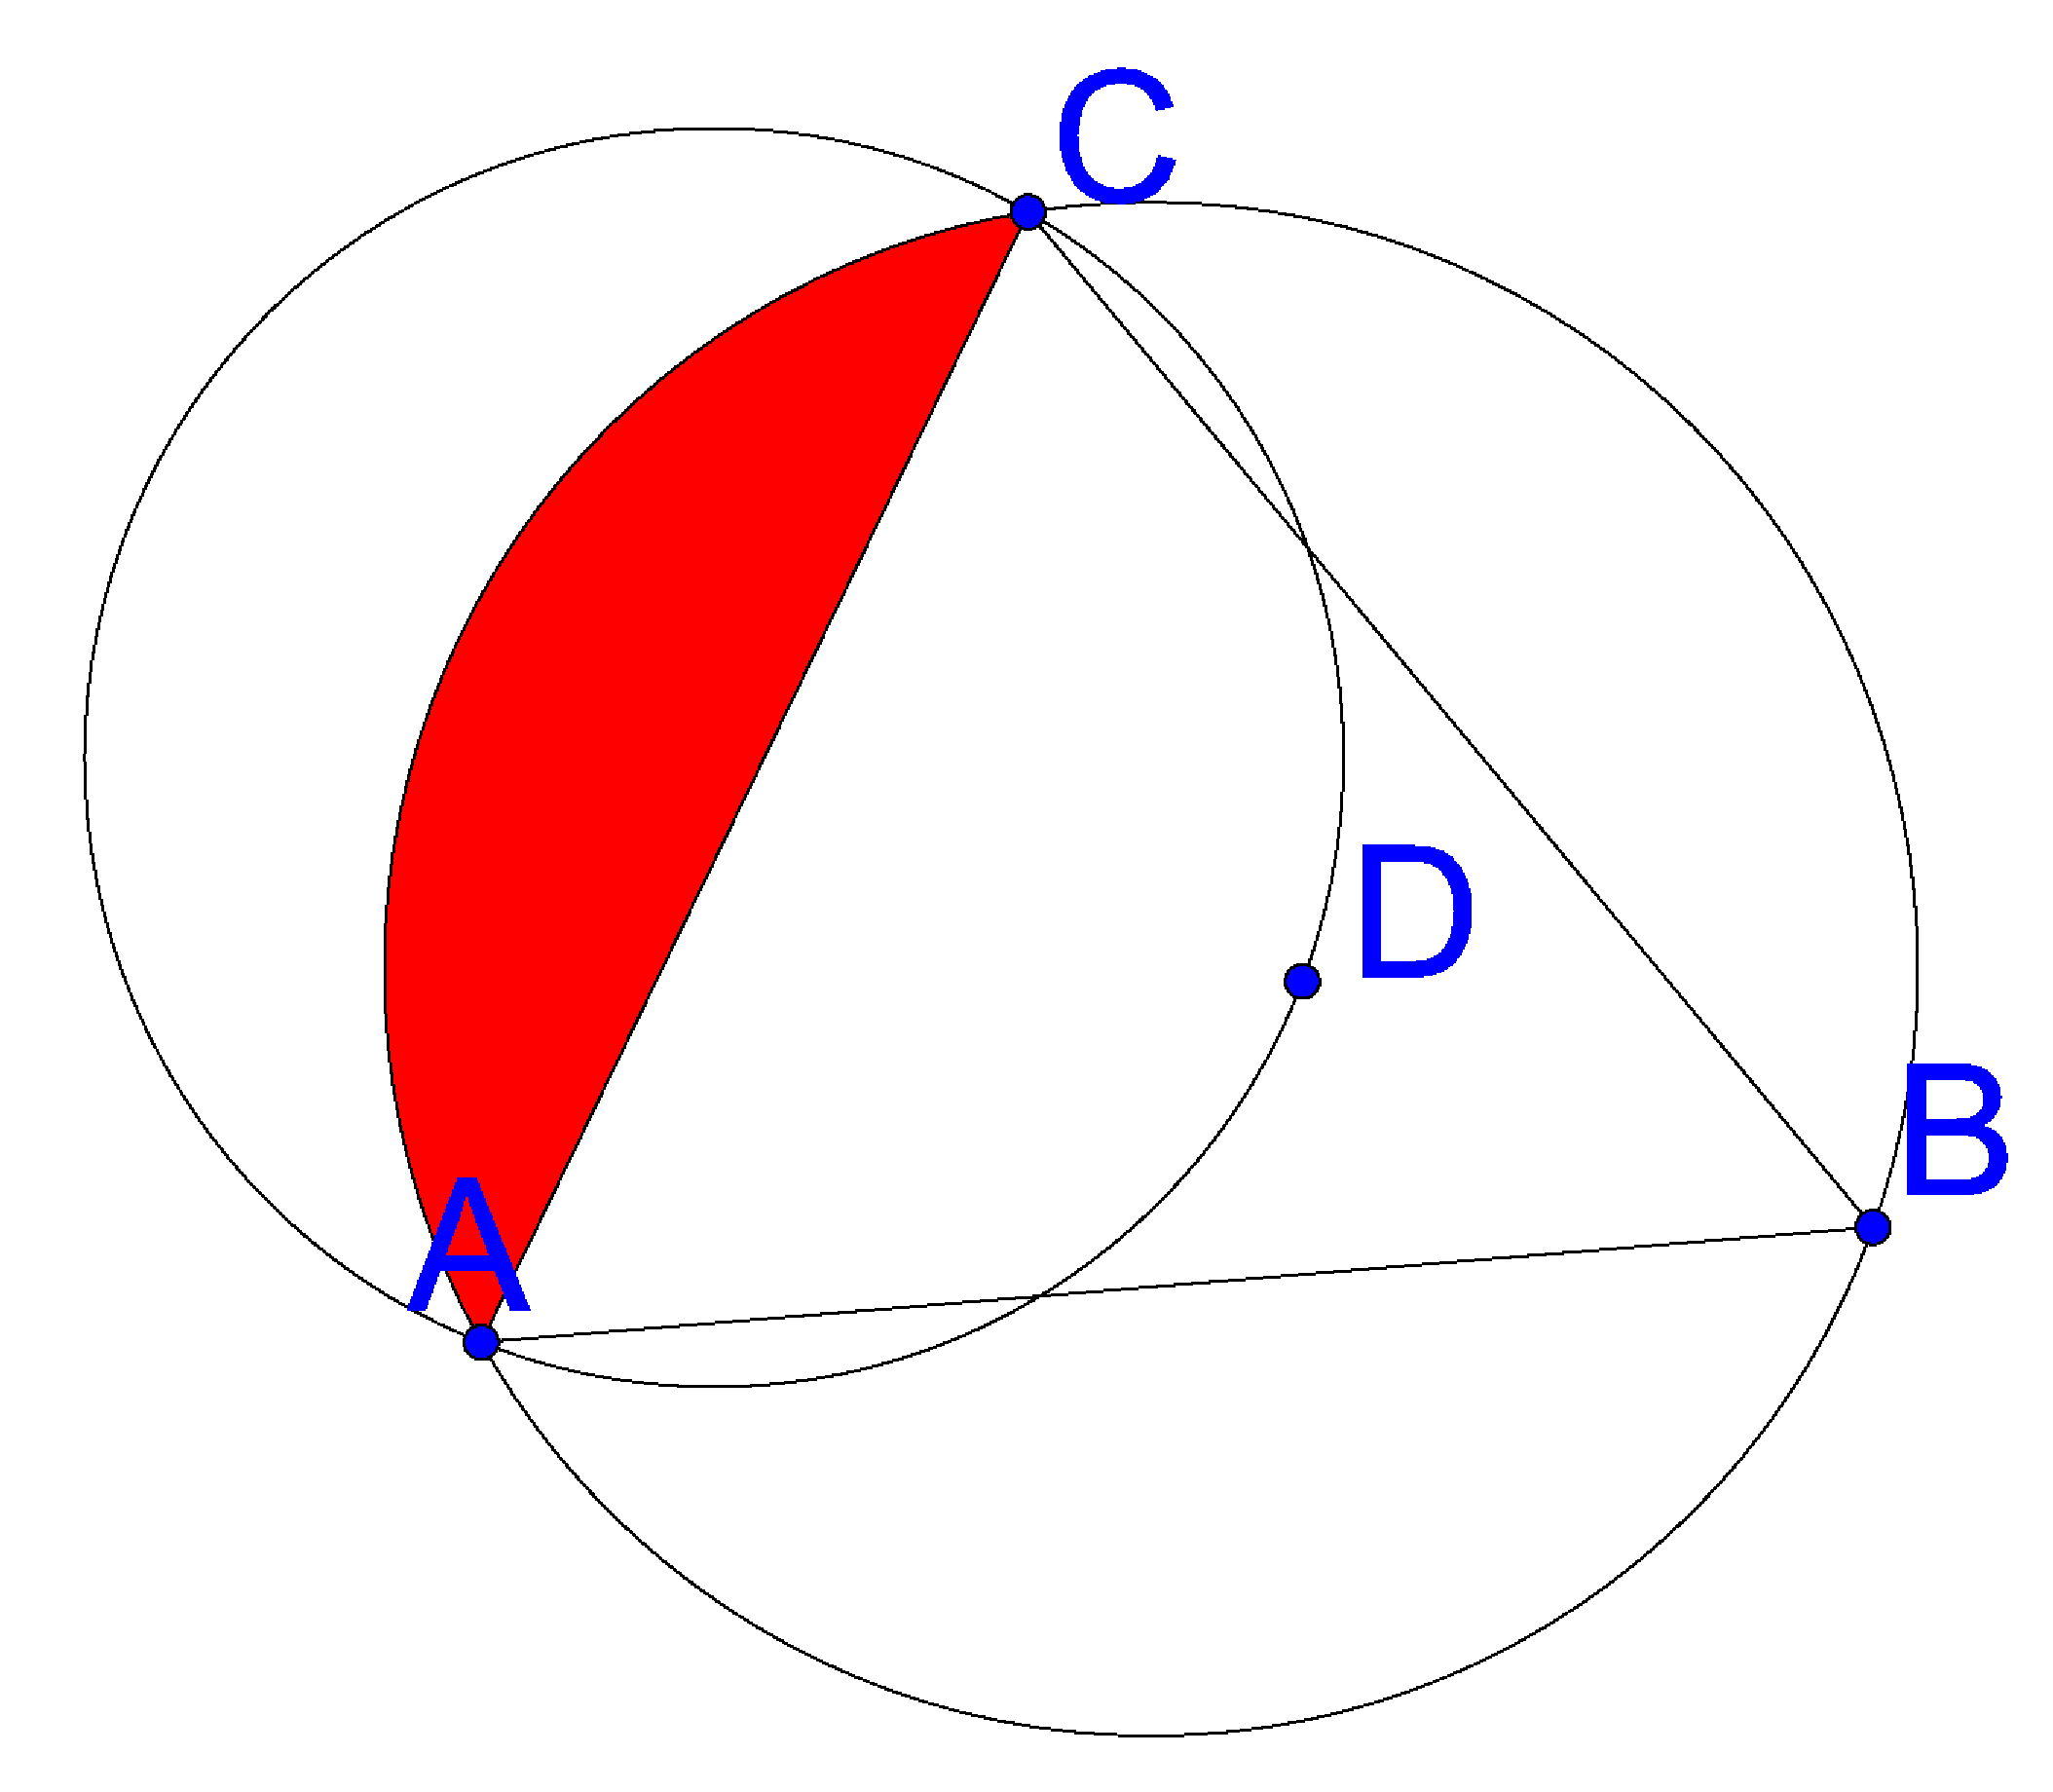
\includegraphics[width=0.2\linewidth]{eps/noPointinRegion.eps}
\caption{The red marked region contains no Points of G because it is always contained in $\bigcirc{ACD} $ which must be empty by definition.}
\label{fig:empty_region}
\end{figure}

Keil and Gutwin \cite{keil} proved the existence of a path between the points $A $ and $B $ and showed that the length of this path is delimited by the length of the arc from $A $ to $B $ on the circle $\bigcirc{ABC} $.
This path connects $A $ and $B $ when no other points of G are inside $\triangle{ABC} $.
The only precondition is that lemma \ref{emptyregion} holds (which it does).
This path is called the \emph{outward path}.
%überleitung

The recursive definition of this path taken from \cite{kanj} is as follows:
\begin{enumerate}
\item \textbf{Base case:} If $AB \in G $, the path consists of edge AB.
\item \textbf{Recursive step:} Otherwise, a point must reside in the region of $(O) $ subtended by chord AB and away from C. 
Let $T $ be such a point with the property that the region of $\bigcirc{ATB} $ subtended by chord $AB $ closer to $T $ is empty. 
We call T an \emph{intermediate point} with respect to the pair of points $(A, B) $.
Let $(O_1) $ be the circle passing through $A $ and $T $ whose center $O_1 $ lies on segment $AO $  and let $(O_2) $ be the circle passing through $B $ and $T $ whose center $O_2 $ lies on segment $BO $.
Then both $(O_1) $ and $(O_2) $ lie inside $(O) $, and $\angle{AO_1T} $ and $\angle{TO_2B} $ are both less than $\angle{AOB} \leq \frac{4\pi}{k} $.
Moreover, the region of $(O_1) $ subtended by chord $BT $ and containing $O_2 $ is empty. Therefore, we can recursively construct a path from $A $ to $T $ and a path from $T $ to $B $, and then concatenate them to obtain a path from A to B.  
\end{enumerate}
Figure \ref{fig:intermediate_point} contains an example for an intermediate point.


\begin{figure}[h!]
\centering
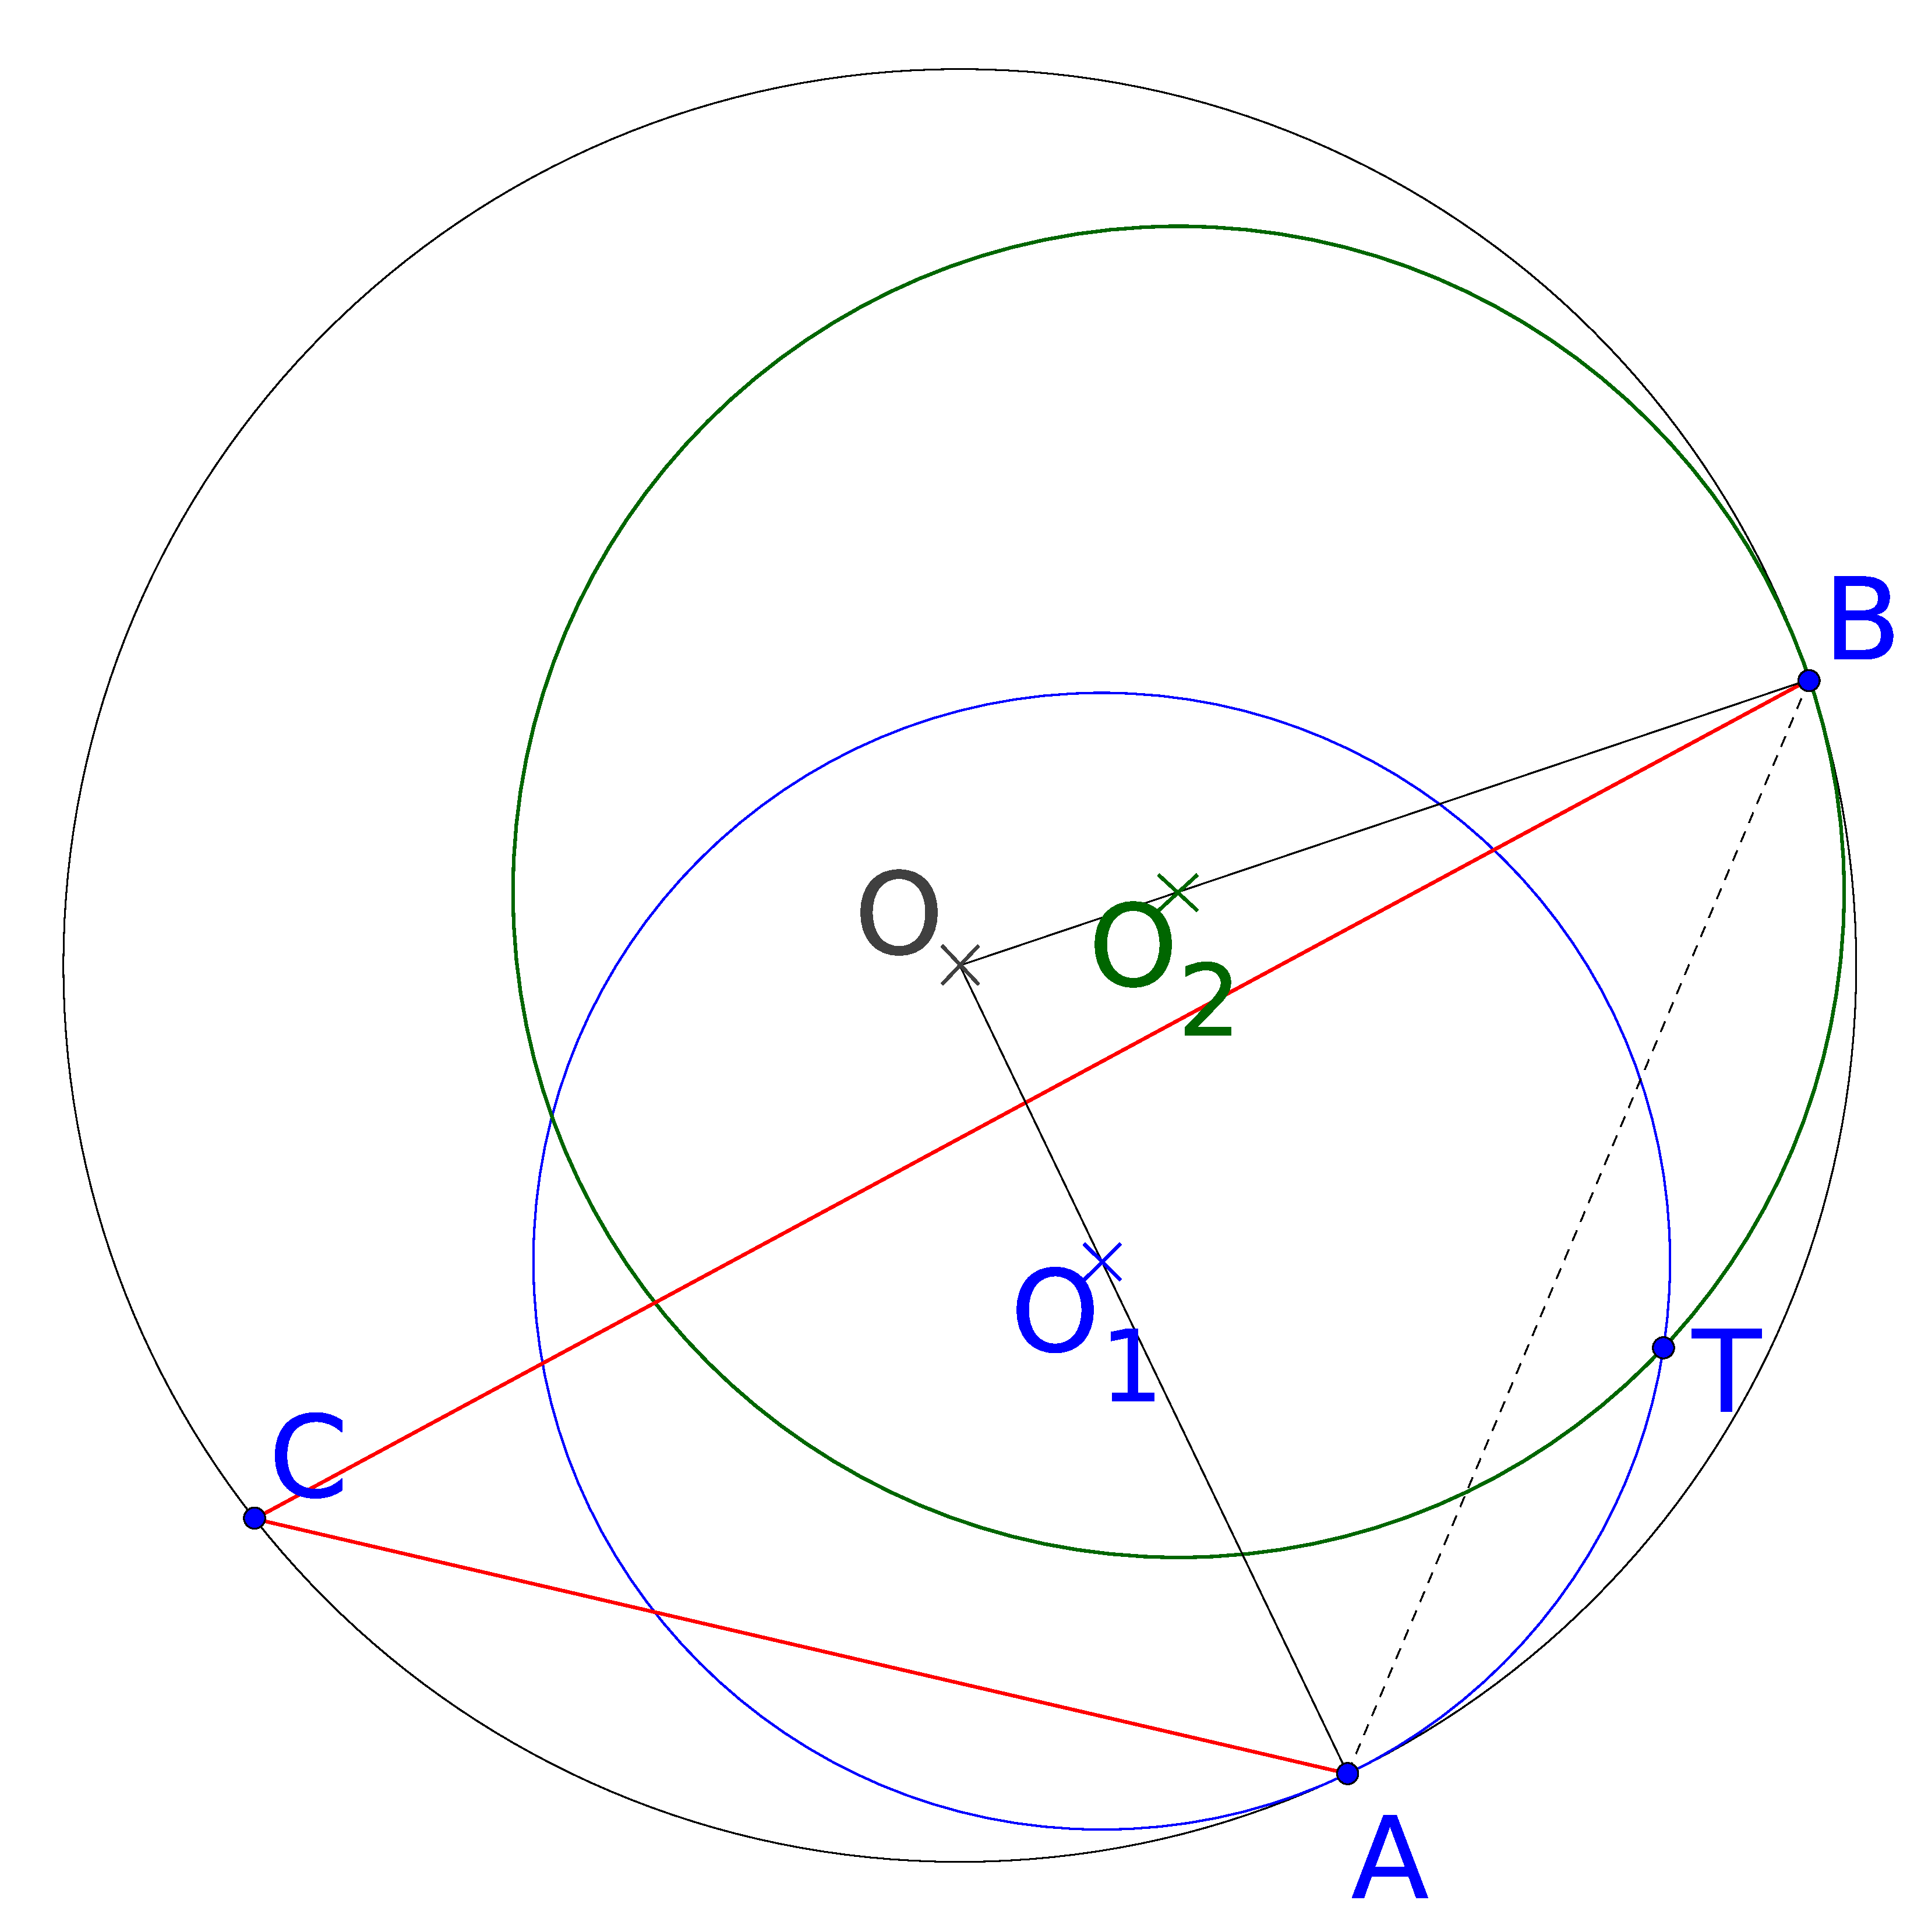
\includegraphics[width=0.5\linewidth]{eps/IntermediatePoint.eps}
\caption{The intermediate point $T $ with respect to pair $(A,B) $, and the circles $O_1 $ and $O_2 $, which are completely within $O $. }
\label{fig:intermediate_point}
\end{figure}


We must proof the following proposition (which is from \cite{kanj}).

\begin{prop}
\label{outward_path}
In every recursive step of the outward path construction described above, if $M_p $ is an intermediate point with respect to a pair of points $(M_i, M_j) $, then:
\begin{enumerate}
\item there is a circle passing through C and $M_p $ that contains no point of G, and
\item circles $\bigcirc{CM_iM_p} $ and $\bigcirc{CM_jM_p} $ contain no points of G, except, possibly, in the region subtended by chords $M_iM_p $ and $M_pM_j $, respectively, away from C.
\end{enumerate}
\end{prop}

\begin{figure}[h!]
\centering
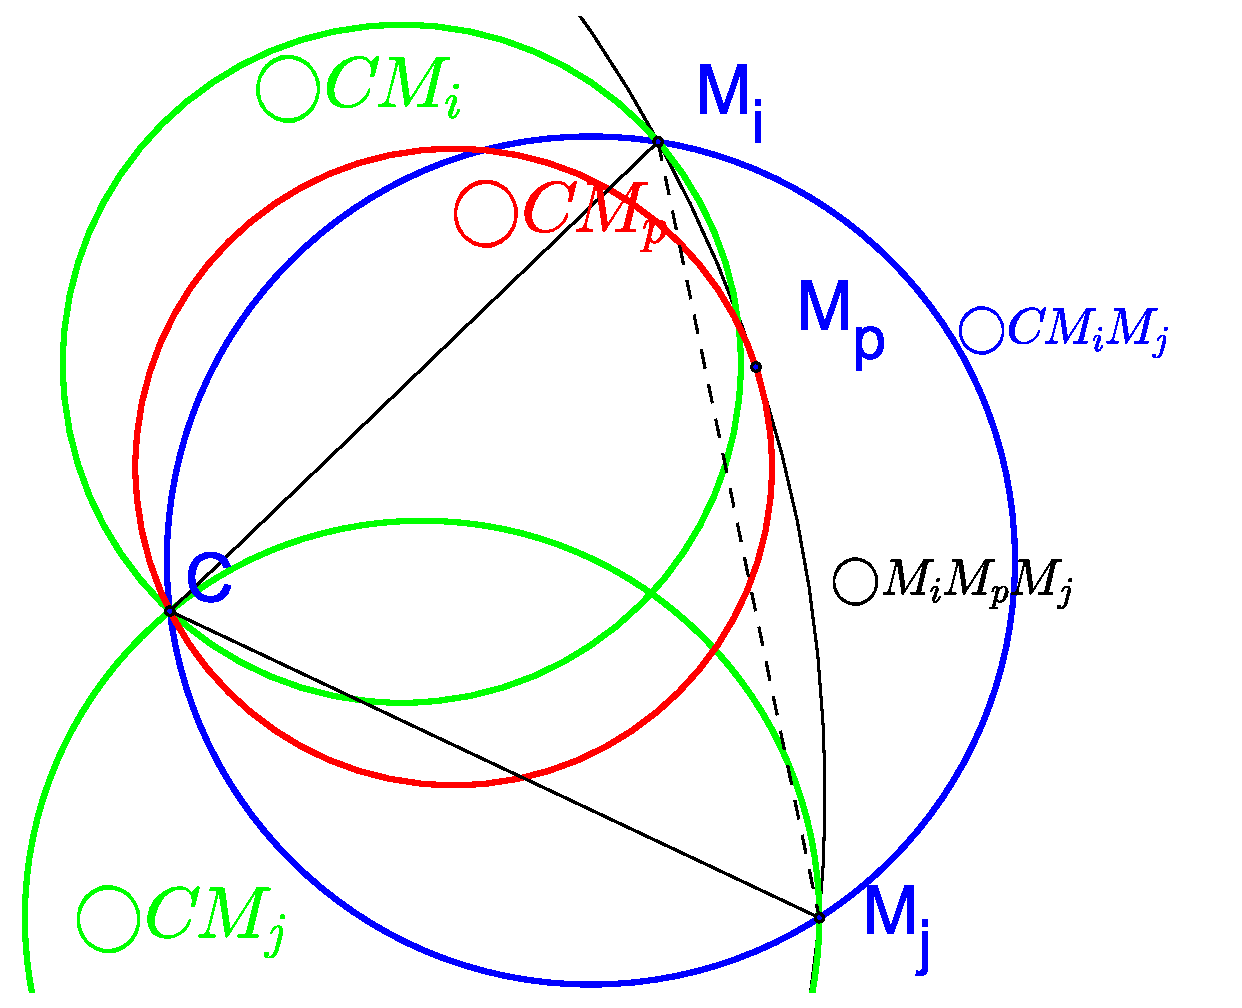
\includegraphics[width=0.9\linewidth]{eps/beweis_outward.eps}
\caption{Example for proof of proposition \ref{outward_path}.}
\label{fig:outward_path_beweis}
\end{figure}

\begin{proof}


Let $G $ be the set of nodes which is created by PDT. 
Since $CA $ and $CB $ are edges in $G $ there are circles $\bigcirc{CM_i} $ and $\bigcirc{CM_j} $ which have $C $ and $M_i $, and $C $ and $M_j $, respectively, on it's border and do not contain any other nodes of $G $. 
At this point I assume, without loss of generality, that $M_i $ and $M_j $ lie on the y-axis of the coordinate system and $C $ lies to the left of these points.
First, notice that $\triangle{CM_iM_j} $ is empty by precondition and the area $R_{\bigcirc{M_iM_pM_j}} $ of $\bigcirc{M_iM_pM_j} $ subtended by chord $M_iM_j $ away from $C $ contains no other points either.
This proof is divided into three cases.
\begin{enumerate}
\item $\bigcirc{CM_p} $ is tangential to $\bigcirc{CM_iM_j} $ at C.
\item $\bigcirc{CM_p} $ overlaps $\bigcirc{CM_iM_j} $ in the upper halfplane subtended by chord $CM_i $ (away from $M_j $).
\item $\bigcirc{CM_p} $ overlaps $\bigcirc{CM_iM_j} $ in the lower halfplane subtended by chord $CM_j $ (away from $M_i $).
\end{enumerate}
Since the two circles $\bigcirc{CM_p} $ and $\bigcirc{CM_iM_j} $ share the point $C $, $\bigcirc{CM_p} $ cannot overlap $\bigcirc{CM_iM_j} $ on both sides of the edge $CM_p $.
For case 1 $\bigcirc{CM_p} $ is completely inside $\bigcirc{CM_iM_j} $ and therefore devoid of any points.
For case 2 $\bigcirc{CM_p} $ is completely inside the area $R_{\bigcirc{M_iM_pM_j}} \cup \bigcirc{CM_iM_j} \bigcirc{CM_i} $ and, therefore, empty.
$\bigcirc{CM_p} $ cannot overlap $\bigcirc{CM_i} $ because of the following lemma.
\begin{lemma}
\label{circles}
If $A $ and $B $ are points in the plane and are located in different halfplanes of a line $CM_i $, and $A $ and $B $ are not allowed to reside inside a circle $\bigcirc{CM_i} $, there is no circle $\bigcirc{ABC} $ which does not contain $M_i $ and overlaps circle $\bigcirc{CM_i} $.
\end{lemma}
\begin{proof}
 Let, without loss of generality, $C $ and $M_i $ be on a line $CM_i $ which is parallel to the y-axis.
$A $ and $B $ are then located to the left and right of this line.
You can see this construction in figure \ref{fig:beweis_circles}.

This proof uses a contradiction. % widerspruchsbeweis  -> Florentin fragen
$A $ cannot reside inside $\bigcirc{CM_i} $, since $CM_i $ is a PDT-edge.
The circle $c_1 $ must not contain $M_i $ and, therefore, must cross the circle $\bigcirc{CM_i} $ in front of $M_i $.
Notice that the next part of the circle $c_1 $ must be inside of circle $\bigcirc{CM_i} $, since we started outside.
Because $c_1 $ must cross $B $ and $B $ lies outside of $\bigcirc{CM_i} $, $c_1 $ crosses a second time $\bigcirc{CM_i} $.
And the last conclusion is that $C $ is a common point of $\bigcirc{CM_i} $ and $c_1 $.
Hence, we have got three intersections of $\bigcirc{CM_i} $ and $c_1 $ at least.
Since $A $ and $B $ lie outside of $\bigcirc{CM_i} $, these two circles are not equal.
But two circles which intersect at least three times and are not equal, do not exist.
\end{proof}
The proof of case 3 works analogously.
These conclusions proof part a) of proposition \ref{outward_path}.

The following part of this work proofs part b) of the same proposition.
The main argument of this proof is that $\bigcirc{CM_iM_p} $ is contained completely in the area $\bigcirc{CM_i} \cup  R_{\bigcirc{M_iM_pM_j}} \cup R2_{\bigcirc{CM_iM_j}} $ with $R2_{\bigcirc{CM_iM_j}} $ being the area of $\bigcirc{CM_iM_j} $ subtended by chord $M_iM_j $ closer to $C $.
I show that every possible position of $\bigcirc{CM_i} $ includes the area $R3_{\bigcirc{CM_iM_p}} $ of $\bigcirc{CM_iM_p} $ subtended by chord $CM_i $ away from $M_j $.
The proof is divided into three cases of how $\bigcirc{CM_i} $ can be located:
\begin{enumerate}
\item $\bigcirc{CM_i} $ is equal to $\bigcirc{CM_iM_p} $.
\item $\bigcirc{CM_i} $ overlaps $\bigcirc{CM_iM_p} $ in the halfplane subtended from line $CM_i $ away from $M_j $.
\item $\bigcirc{CM_i} $ overlaps $\bigcirc{CM_iM_p} $ in the halfplane subtended from line $CM_i $ closer to $M_j $.
\end{enumerate}
First, assume, without loss of generality, that $C $ and $M_i $ lie on a horizontal line and $M_j $ is located below this line.
$\bigcirc{CM_iM_p} $ can only overlap $\bigcirc{CM_i} $ on one side of line $CM_i $, since they share these two points.

For case 1, since $\bigcirc{CM_i} $ is empty, $\bigcirc{CM_iM_p} $ must be empty, too.

For case 2, $\bigcirc{CM_i} $ moves up, away from $M_j $, expanding the area in the same direction of which $R3_{\bigcirc{CM_iM_p}} $ is located.
So, $R3_{\bigcirc{CM_iM_p}} $ cannot overlap $\bigcirc{CM_i} $ in this case.

Case 3, the only case where $R3_{\bigcirc{CM_iM_p}} $ would overlap $\bigcirc{CM_i} $, cannot occur, since $M_p \in G $ and $M_p $ is, obviously, located on $\bigcirc{CM_iM_p} $.
So, if $\bigcirc{CM_i} $ moves down, towards $M_j $, it would contain $M_p $, which cannot happen, since $\bigcirc{CM_i} $ is a PDT-circle. 

Notice that the proof for $\bigcirc{CM_jM_p} $ works analogously substituting $M_i $ with $M_j $ and vice versa.
 
\end{proof}
\begin{figure}[h!]
\centering
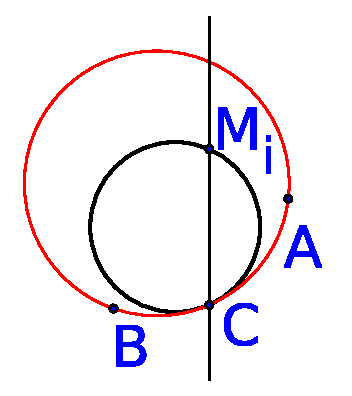
\includegraphics[width=0.5\linewidth]{eps/beweis_circles.eps}
\caption{Example of the construction of lemma \ref{circles}.}
\label{fig:beweis_circles}
\end{figure}
Another lemma we need in order to proof proposition \ref{mastertheorem} is the following:
\begin{lemma}
\label{outward_3}
If four points $A $, $B $, $C $ and $M_1 $ are on one circle and $C $ and $M_1 $ are on different halfplanes of chord $AB $, then $\angle{AM_1B} + \angle{ACB} =\pi $ is true (see figure \ref{fig:winkel_fuer_outward_3} for an graphical illustration of this lemma).
\end{lemma}
\begin{proof}
see Euklid, book 3, Proposition 22.  (Nochmal besprechen)


\begin{figure}[h!]
\centering
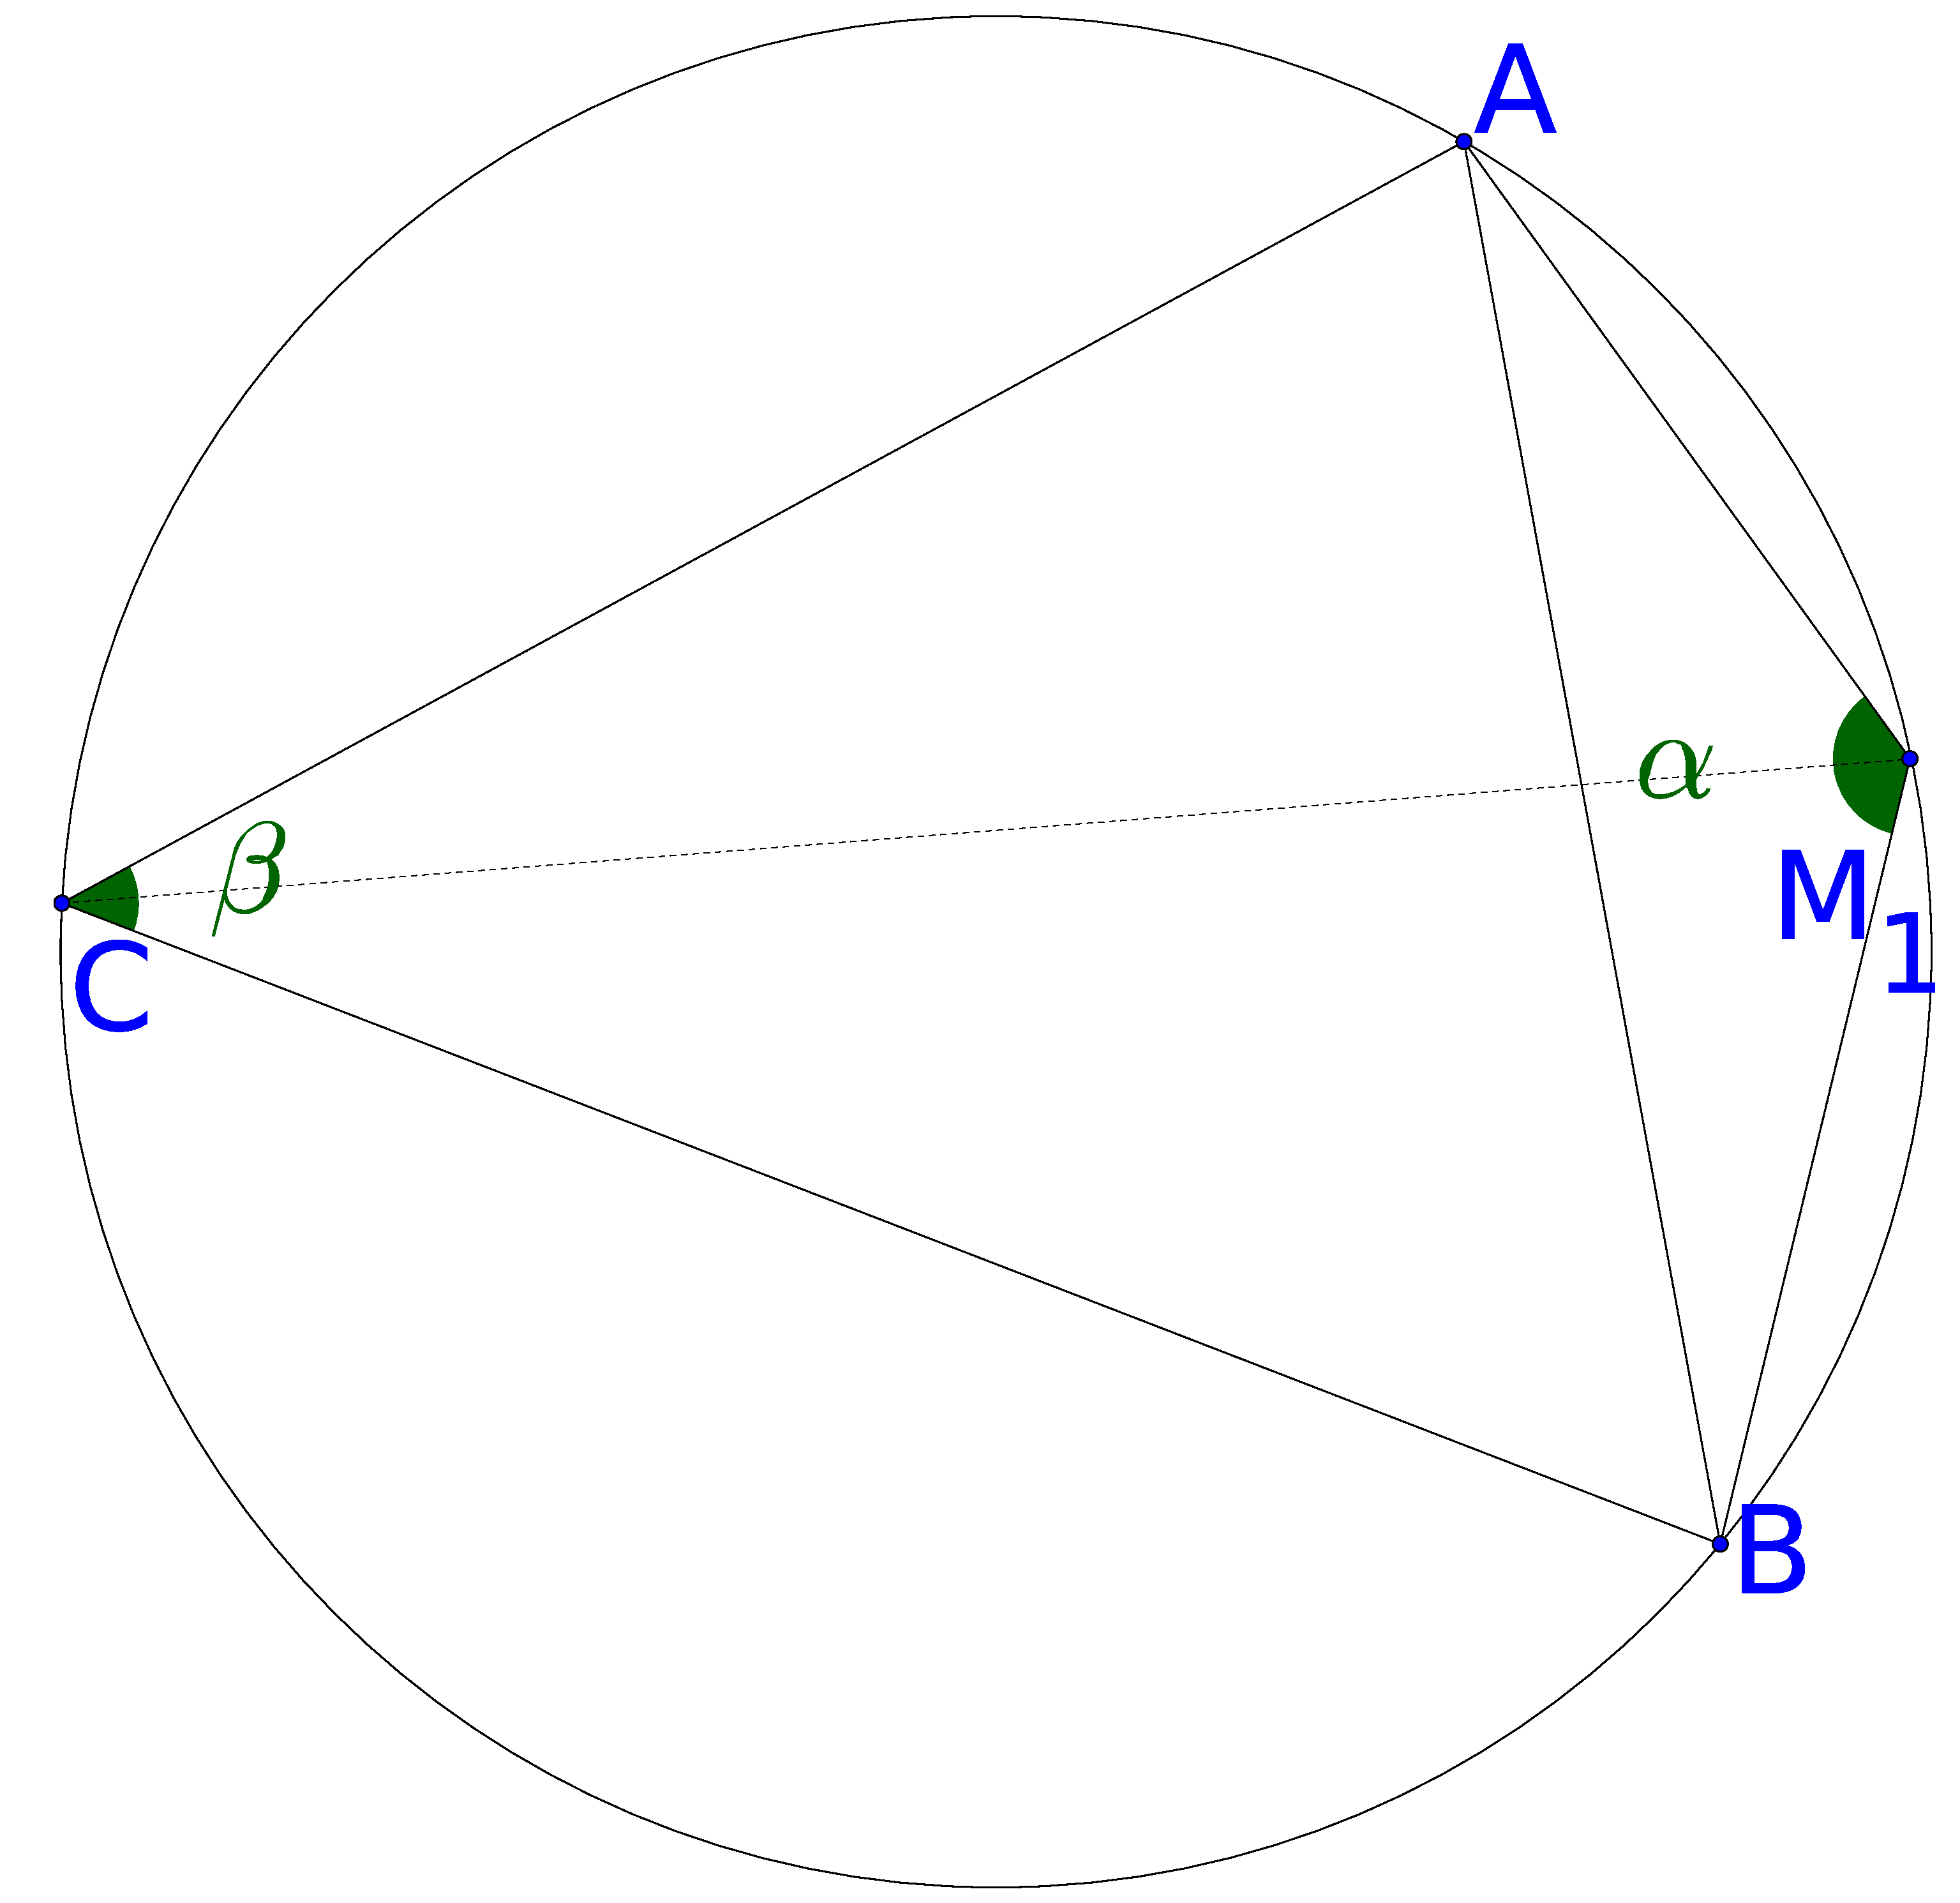
\includegraphics[width=0.4\linewidth]{eps/Winkel_fuer_outward_3.eps}
\caption{Example for lemma \ref{outward_3} }
\label{fig:winkel_fuer_outward_3}
\end{figure}
\end{proof}
Now, we can proof the following lemma from \cite{kanj}, which shows, that for the case of the outward path, proposition \ref{mastertheorem} is satisfied:

\begin{lemma}
Let $k \geq 14$ be an integer, and let $CA $ and $CB $ be edges in $G $ such that $\angle{BCA} \leq \frac{2\pi}{k} $ and $CA $ is the shortest edge in the angular sector $\angle{BCA} $. There exists a path $p : A=M_0, M_1, \dotsc, M_r=B $ in $G $ such that:
\begin{enumerate}
\renewcommand{\labelenumi}{(\roman{enumi})}
\item $|CA| + \sum_{i=0}^{r-1}|M_iM_{i+1}| \leq (1+2\pi(k \cos(\frac{\pi}{k}))^{-1})|CB|$
\item There is no edge in $G $ between any pair $M_i $ and $M_j $ lying in the closed region delimited by $CA, CB $ and the edges of $p $, for any $i $ and $j $ satisfying $0 \leq i < j -1 \leq r $.
\item $\angle{M_{i-1}M_iM_{i+1}} > \pi - \frac{2\pi}{k} $, for $i=1,\dotsc,r-1 $.
\item $\angle{CAM_1} \geq \frac{\pi}{2} - \frac{pi}{k} $.
\end{enumerate}	 
\end{lemma}

\begin{proof}
This proof is performed almost equal to \cite{kanj}, but covering more details.
%and $\sin{\theta} = \frac{|AB|}{2|OA|}) $
\renewcommand{\labelenumi}{(\roman{enumi})}%
\begin{enumerate}
\item 
\begin{equation*}
\begin{split}
|CA|+|\overarc{AB}| &= |CB| + 2\theta \cdot |OA| \\
&\stackrel{a)}{=}|CB| + (\frac{\theta}{\sin{\theta}})\cdot |AB| \\
&\stackrel{b)}{=} |CB| + (\frac{\theta}{\cos{\frac{\theta}{2}}}) \cdot |CB|\\
&\stackrel{c)}{\leq} (1+2\pi(k \cos{\frac{\pi}{k}})^{-1}) |CB|  
\end{split}
\end{equation*}
Since $|CA| \leq |CB| $, $|CA|+|\overarc{AB}| $ is largest, when $CA $ and $CB $ are symmetrical to the diameter of $\bigcirc{ABC} $, we can assume $|CA|=|CB| $.
$|\overarc{AB}| $ can be replaced with $2\theta \cdot |OA| $ (angle times radius).
For every chord $s $ of a circle $(c) $ it is true, that $s=2r\sin{\frac{\alpha}{2}} $, with $r $ being the radius of $(c) $ and $\alpha $ being the angle between the endpoints of $s $ in middlepoint $c $ facing $s $.
Note that $\alpha = 2\theta $. 
These equations proof a).

Next, substitute $|AB| $ with $|AB| = \sin{\frac{\theta}{2}} \cdot 2|CB| $ and replace $\sin{\theta} $ with the trigonometry identity $\sin{\theta}=2\sin{\frac{\theta}{2}} \cos{\frac{\theta}{2}} $.
You receive equation b).

At last, substitute $\theta $ using inequality $\theta \leq \frac{2\pi}{k} $ with $k > 2 $, obtaining c).

\item  Suppose, $M_i $ and $M_j $ is an edge in $G $, then there exists a circle with these two points on it's border which does not contain any other node of $G $.
So, $M_p $ must lie outside of this circle.
By proposition \ref{outward_path} part a) there is a circle $\bigcirc{CM_p} $ trough $C $ and $M_p $ which is empty.
These two last observations contradict each other, since $\bigcirc{M_iM_j} $ would always contain $M_p $.
If $M_p $ does not reside in the circle $\bigcirc{M_iM_j} $, this circle and the circle $\bigcirc{CM_p} $ would cross at least three times (and are not equal), which cannot exist.

\item Since the angles $\alpha $ and $\beta $ between opposite points of a chord in a rectangle which corners lie on a circle are supplementary, this is a fact: $\angle{AM_1B}=\pi - \angle{ACB} $ (see lemma \ref{outward_3} for more details).
The angle $\angle{M_{i-1}CM_{i+1}} $ is smallest, if $M_{i-1} $ and $M_{i+1} $ lie on the circle. 
Note, by precondition we assume $\angle{BCA} \leq \frac{2\pi}{k} $.
These facts proof following inequalities:
\begin{equation*}
\begin{split}
 \angle{M_{i-1}M_iM_{i+1}}&\geq \pi - \angle{M_{i-1}CM_{i+1}}\\
 &\geq \pi - \angle{BCA} \\ &\geq \pi - \frac{2\pi}{k}\\
\end{split}
\end{equation*}



 %http://www.regentsprep.org/regents/math/geometry/gp15/circleangles.htm
\item Since $M_1 $ is inside the area subtended by chord $AB $ from $\bigcirc{ABC} $ \emph{away} from $C $, it is true that $\angle{CAM_1} \geq \angle{CAB} \geq \frac{\pi}{2} -\frac{\pi}{k} $.
The last inequality is true because:
 \begin{equation*}
  \begin{split}
   \angle{CAB}+\angle{ABC}+\underbrace{\angle{BCA}}_{\leq \frac{2\pi}{k}}&=\pi\\
   \angle{CAB}+\angle{ABC} &\geq \pi - \frac{2\pi}{k} \\
   \angle{CAB} &\geq \frac{\pi-\frac{2\pi}{k}}{2}=\frac{\pi}{2}-\frac{\pi}{k}
   \end{split} 
\end{equation*}
Since $CA \leq CB $, $\angle{CAB} $ can be at most the half of $\pi - \frac{2\pi}{k} $, proving the last inequality.

\end{enumerate}
\end{proof}

 
%\begin{figure}[h!]
%\centering
%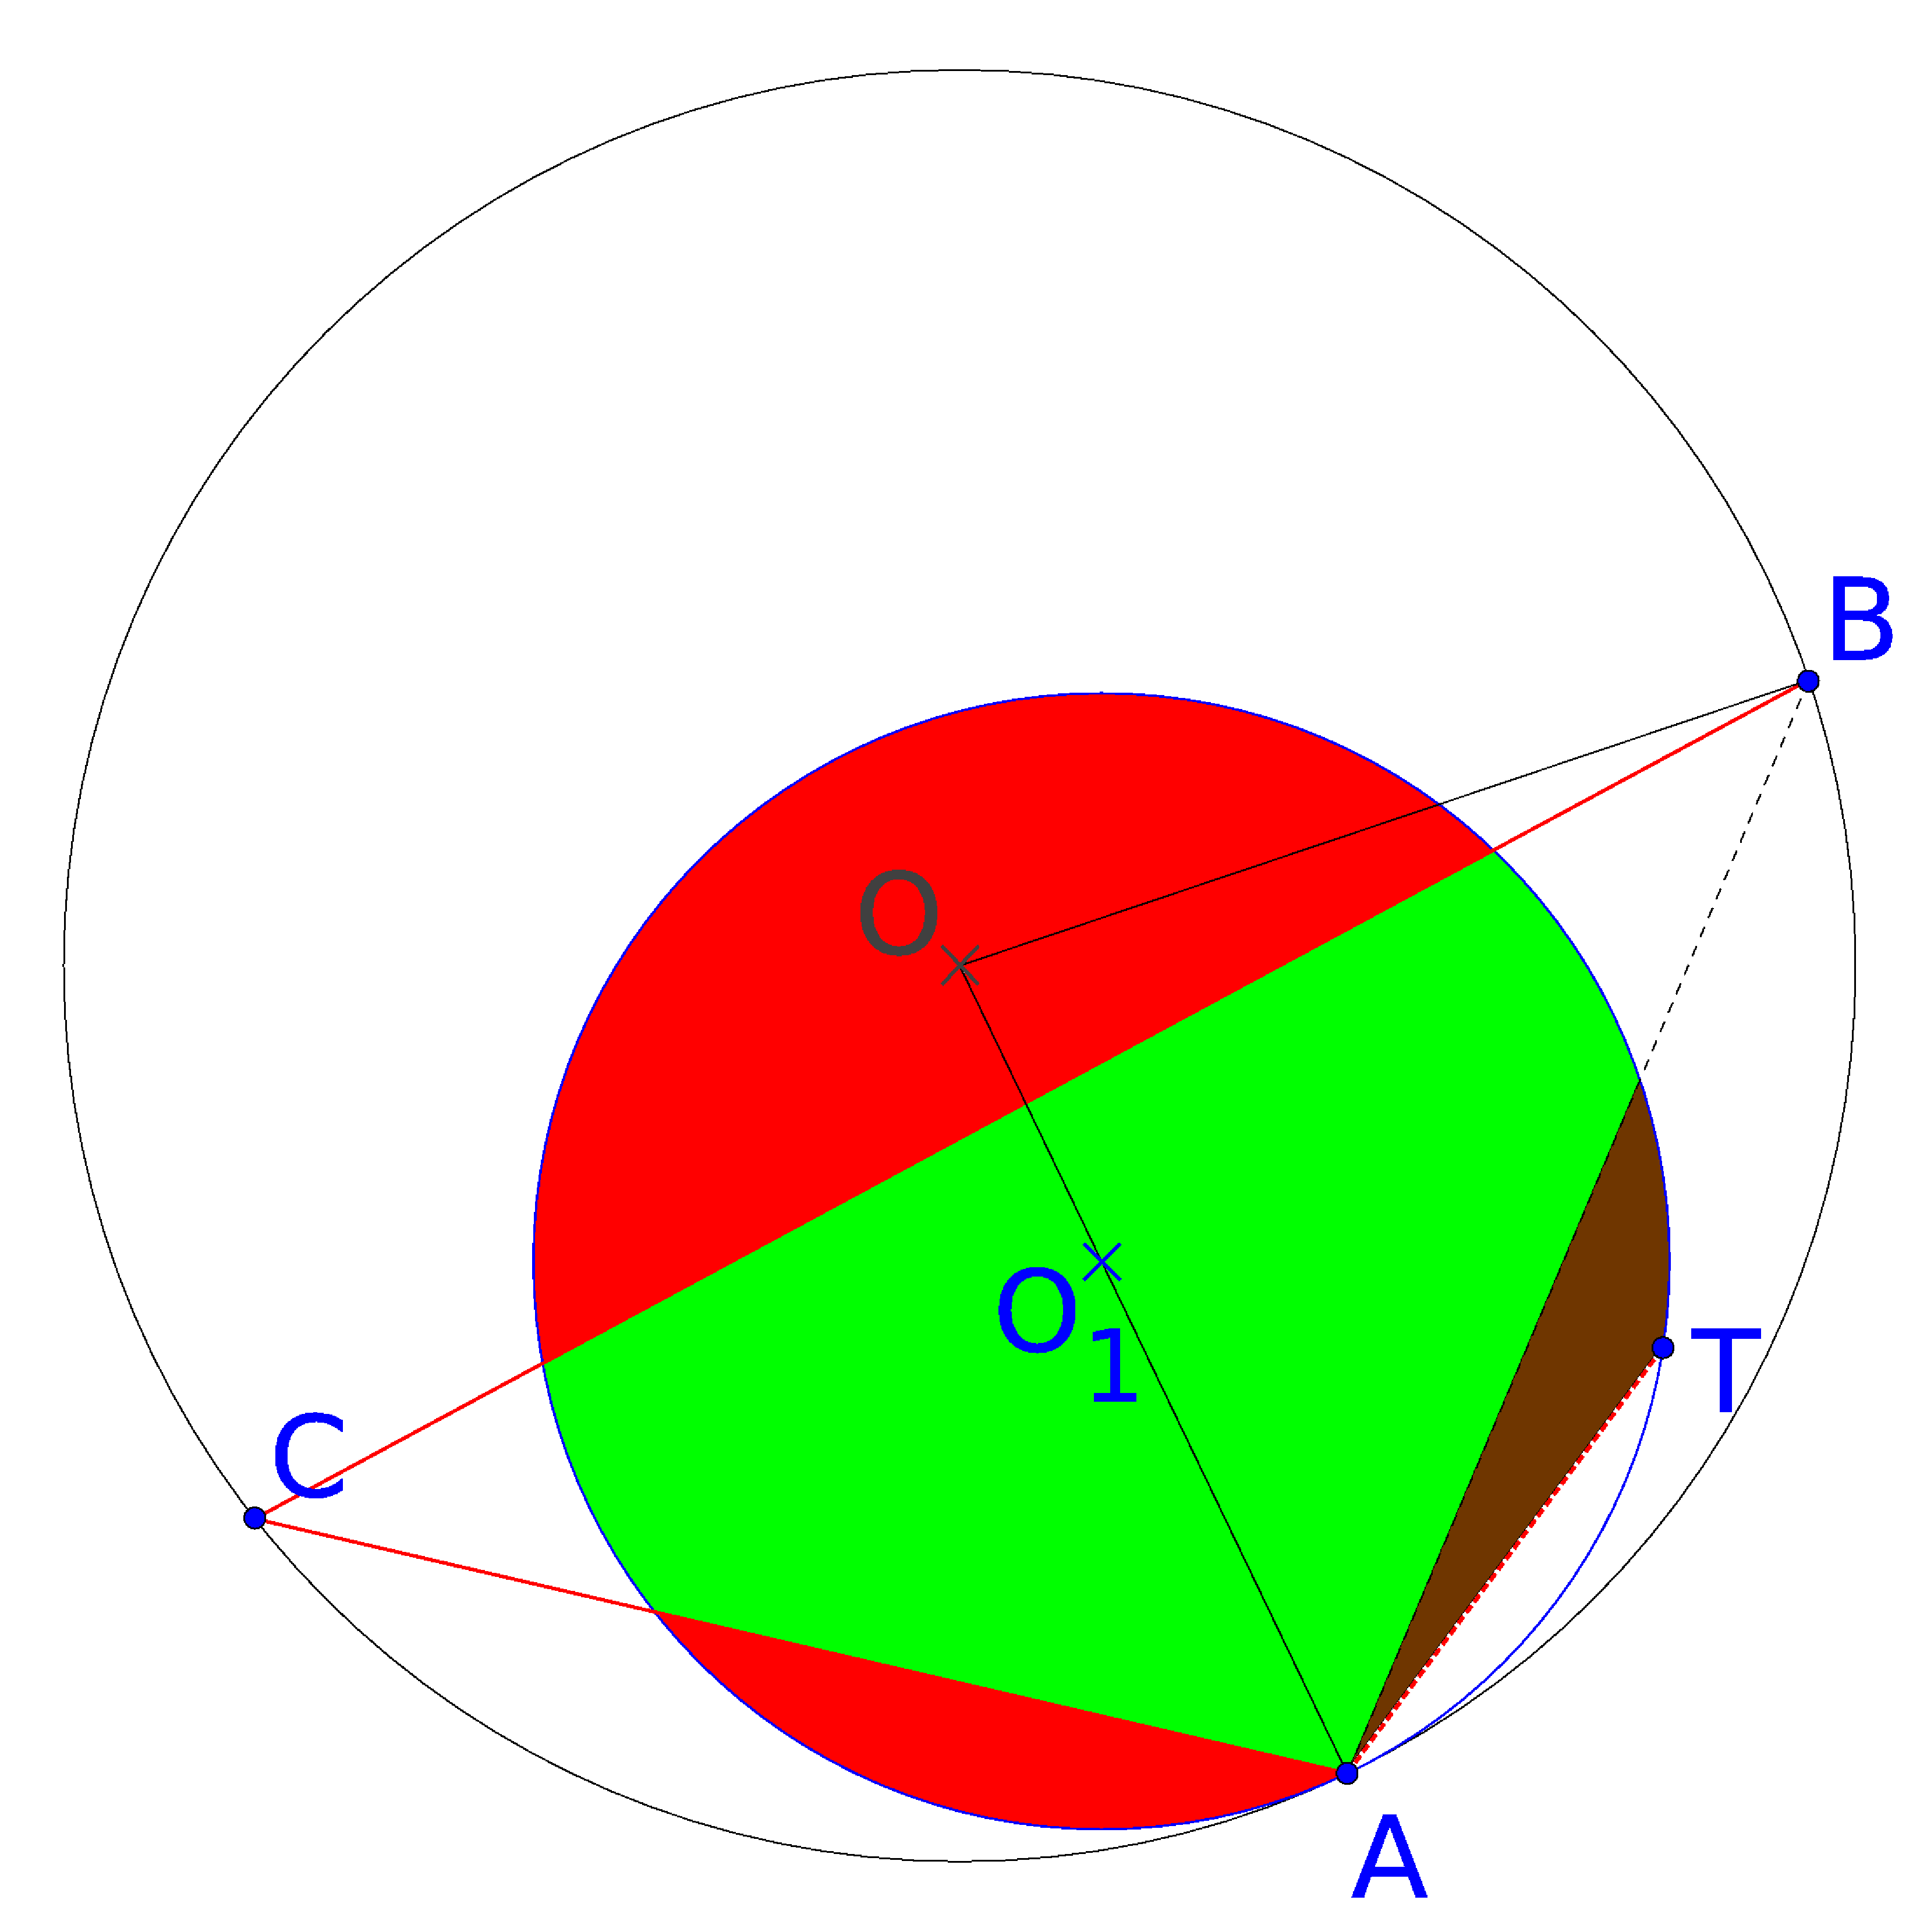
\includegraphics[width=0.5\linewidth]{eps/IntermediatePoint_beweis.eps}
%\caption{The red regions must be empty by lemma \ref{emptyregion}, the green area is empty by precondition and the brown region must be empty by ... }
%\label{fig:intermediate_point_beweis}
%\end{figure}
%
%
%\begin{enumerate}
%\item $|CA| + \sum\nolimits_{i=0}^{r-1} |M_iM_{i+1}| \leq (1+2\pi (k*\cos{\frac{\pi}{k}})^{-1})|CB| $
%\item There is no edge in G between any pair $M_i $ and $M_j $ lying in the closed region delimited by CA, CB and the edges of p, for any i and j satisfying $0 \leq i < j-1 \leq r $ 
%\item $\angle{M_{i-1}M_iM_{i+1}} > \frac{k-2}{k}\pi $, for $i=1, ..., r-1 $ 
%\item $\angle{CAM_1} \geq \frac{\pi}{2}-\frac{\pi}{k} $
%\end{enumerate}




\subsection{inward Path}
Now, we perform the proof for the case when $\triangle{ABC} $ contains other nodes.

Let $S $ be the set of points which contains points $A $ and $B $, and all the points interior to $\triangle{ABC} $ excluding $C $.
Then $CH(S) $ are all the points which are on the convex hull of $S $.
Let these points be called $N_0=A $ and $N_t=B $ and points $N_1 , \cdots ,N_{t-1} $ are the points on $CH(S) $ which lie inside $\triangle{ABC} $. 
The following proposition is taken from \cite{kanj}:
\begin{prop}
\label{inward_pre}
For every $i=1, \cdots, t-1: $
\begin{enumerate}
\renewcommand{\labelenumi}{\alph{enumi})}
\item $CN_i \in G $,
\item $|CN_i| \leq |CN_{i+1}| $, and
\item  $\angle{N_{i-1}N_iN_{i+1}} \geq \pi $, where $\angle{N_{i-1}N_iN_{i+1}} $ is the angle facing point $C $.
\end{enumerate} 
\end{prop}
\begin{proof}
Since $CA $ is the shortest edge in the angular sector $\angle{BCA} $, $|CA| \leq CN_i , for i=1 ,\cdots, t-1 $  and since $N_1 , \cdots, N_t $ are on $CH(S) $, b) is true.

Part c) follows from the convexity of $CH(S) $. All interior angles to $CH(S) $ measure at most $\pi $, so all the exterior angles fulfil $\angle{N_{i-1}N_iN_{i+1}}\geq \pi $ 
\end{proof}

Since $CN_i \leq CN_{i+1} $ and no other point of $G $ lies inside $\triangle{N_iCN_{i+1}} $, $CN_i $ is the shortest edge in the angular sector $\angle{N_iCN_{i+1}} $.